\chapter{Géométrie de l’Univers en expansion}

Il s’agit de l’Univers en expansion et de sa géométrie. L’objectif est de décrire ce que signifie l’expansion de l’espace avant de se demander ce qui la provoque. La cosmologie newtonienne \(F=ma\) viendra ensuite, puis la géométrie et la dynamique seront réunies dans le cadre complet de Friedmann--Robertson--Walker.

\section{Coordonnées comobiles sur une ligne en expansion}

Commençons par l’exemple le plus simple qui soit : un espace à une dimension, et non un espace-temps. Imaginons une droite infinie sur laquelle des galaxies sont régulièrement espacées. La coordonnée \(x\) ne mesure pas encore une distance physique. Elle sert à repérer les galaxies. On peut voir \(x\) comme le nom d’une galaxie, un nom qui lui reste attaché même si toute la configuration s’étire ou se contracte.

Soit \(a\) la distance physique entre la galaxie appelée \(x=0\) et celle appelée \(x=1\). Alors, la distance physique entre deux galaxies quelconques est
\begin{equation}
d=a\,\Delta x.
\end{equation}
La différence de coordonnées \(\Delta x\) est simplement la différence entre leurs repères. Le facteur \(a\) transforme cette différence de repères en une distance réelle, mesurée à l’aide de règles graduées en mètres.

Imaginons maintenant que la droite soit un fil élastique que l’on étire. Les repères restent attachés aux galaxies, mais la distance entre galaxies voisines varie au cours du temps. La même relation devient
\begin{equation}
d(t)=a(t)\,\Delta x.
\end{equation}
À ce stade, l’homogénéité signifie simplement que les galaxies voisines sont partout également espacées, même si cet espacement commun peut varier au cours du temps.

\section{Loi de Hubble et absence de centre}

Pour déterminer la vitesse relative de deux galaxies fixes, considérons la même paire de galaxies, de sorte que \(\Delta x\) ne varie pas au cours du temps. En dérivant, on obtient
\begin{align}
\dot d &= \dot a\,\Delta x \\
       &= \frac{\dot a}{a}\,a\,\Delta x \\
       &= \frac{\dot a}{a}\,d.
\end{align}
Définissons
\begin{equation}
H(t)\equiv \frac{\dot a}{a},
\end{equation}
alors
\begin{equation}
\dot d = H(t)\,d.
\end{equation}
C’est la loi de Hubble.

L’expression historique ``constante de Hubble'' est trompeuse. Cette quantité est constante dans l’espace, mais pas dans le temps. À un instant donné, elle a la même valeur pour toutes les galaxies, mais, en général, elle varie au cours de l’évolution de l’Univers. Il vaut mieux la considérer comme le paramètre de Hubble.

Cette loi indique que les galaxies les plus éloignées s’éloignent plus rapidement. Elle ne désigne aucun centre. Rien dans le raisonnement ne privilégie \(x=0\), ni aucun autre point. Tous les observateurs voient la même règle. Dans ce modèle, l’expansion de l’Univers n’est donc pas une explosion partie d’un lieu privilégié.

Le décalage vers le rouge intervient immédiatement. Si deux galaxies échangent des signaux lumineux alors qu’elles s’éloignent l’une de l’autre, la lumière reçue est décalée vers le rouge. Plus la vitesse d’éloignement est grande, plus ce décalage est important. Les raies spectrales nous renseignent donc sur les vitesses d’éloignement. Les distances sont plus difficiles à mesurer, et les premières estimations de Hubble étaient approximatives. Son premier graphique ne formait pas une droite parfaite, mais un nuage de points très dispersés et entachés de grandes incertitudes. Malgré cela, le principe géométrique résistait au bruit : la vitesse d’éloignement est proportionnelle à la distance.

\begin{classroomqa}\audiencequestion{Si les galaxies sont suffisamment éloignées, la loi de Hubble implique-t-elle qu’elles se déplacent plus vite que la lumière ?}\lecturetimestamp{00:20:23}\lecturerresponse{Oui, c’est bien le cas au sens de la vitesse d’éloignement. Ce que vous dites est juste. Nous y reviendrons certainement. C’est l’un des points les plus importants.}\end{classroomqa}

\section{Dimensions supérieures, isotropie et dépendance temporelle de \(a(t)\)}

Rien d’essentiel ne change lorsqu’on ajoute des dimensions spatiales. En deux dimensions, imaginons un quadrillage de galaxies repérées par \((x,y)\), et en trois dimensions, par \((x,y,z)\). Ces coordonnées sont, là encore, des repères comobiles. Elles accompagnent les galaxies au lieu de mesurer directement les distances physiques.

Pourquoi l’espacement dans la direction \(x\) serait-il le même que dans la direction \(y\) ? La réponse est observationnelle. Si les galaxies étaient systématiquement plus concentrées dans une direction que dans une autre, le ciel présenterait un aspect différent selon la direction où l’on regarde. À suffisamment grande échelle, ce n’est pas le cas. Cette uniformité selon la direction est l’isotropie.

En deux dimensions, la distance entre deux galaxies est
\begin{equation}
d=a\sqrt{(\Delta x)^2+(\Delta y)^2},
\end{equation}
et, en trois dimensions,
\begin{equation}
d=a\sqrt{(\Delta x)^2+(\Delta y)^2+(\Delta z)^2}.
\end{equation}
Pour une paire fixe de galaxies, les différences de coordonnées restent constantes ; en dérivant à nouveau, on obtient donc
\begin{equation}
\dot d=\frac{\dot a}{a}\,d.
\end{equation}
La loi de Hubble ne change pas.

L’homogénéité signifie que les choses sont les mêmes d’un endroit à l’autre. L’isotropie signifie qu’elles sont les mêmes quelle que soit la direction. Ni l’une ni l’autre n’est exacte à petite échelle. La vue à travers la Voie lactée diffère de celle qu’on a en regardant hors de son plan, et les galaxies individuelles ne sont pas réparties uniformément à courte distance. Mais après avoir moyenné sur de nombreuses galaxies, l’Univers à grande échelle paraît approximativement semblable en tout lieu et dans toutes les directions.

\begin{classroomqa}\audiencequestion{Si la vitesse est proportionnelle à la distance et que celle-ci augmente, cela signifie-t-il qu’une paire fixe de galaxies doit s’éloigner de plus en plus vite ?}\lecturetimestamp{00:40:22}\lecturerresponse{Non. La loi de Hubble dit qu’à un instant donné, la vitesse d’éloignement est proportionnelle à la distance. À elle seule, elle ne dit pas si la vitesse d’une paire fixe augmente ou diminue au cours du temps. Cela dépend de l’évolution détaillée de \(a(t)\). Si \(a(t)\propto t\), les galaxies voisines s’éloignent à vitesse constante. Si \(a(t)\propto t^2\), la vitesse d’éloignement d’une paire fixe augmente au cours du temps. Si \(a(t)\propto \log t\), elle diminue. La loi \(\dot d=(\dot a/a)d\) est toujours vraie en fonction de la distance, mais l’accélération et la décélération sont des questions distinctes.}\end{classroomqa}

Pendant longtemps, les cosmologistes ont pensé que l’Univers devait être en décélération, puisque la gravité devrait ralentir une expansion initiale, comme elle ralentit un objet lancé vers le haut. Ici, le seul point à retenir est que la loi de Hubble ne détermine pas à elle seule l’évolution de \(\dot a\) ou de \(\ddot a\).

\begin{classroomqa}\audiencequestion{Comment fixe-t-on la valeur initiale du facteur d’échelle \(a\) ?}\lecturetimestamp{00:46:18}\lecturerresponse{Sa normalisation globale est arbitraire. Ce qui a un sens physique, ce n’est pas la valeur numérique de \(a\) à elle seule, mais la façon dont elle varie. Si l’on définit un autre facteur d’échelle \(b=3a\), alors \(\dot b/b=\dot a/a\). Multiplier \(a\) par une constante revient à changer de convention ou d’unités, et non à modifier le paramètre de Hubble.}\end{classroomqa}

\section{De la métrique spatiale à la métrique de l’espace-temps}

Remplaçons maintenant \(\Delta x\) par \(dx\). La distance physique entre deux points voisins est
\begin{equation}
ds=a\,dx,
\end{equation}
d’où
\begin{equation}
ds^2=a^2\,dx^2.
\end{equation}
C’est la métrique spatiale en une dimension. Le coefficient de \(dx^2\) est
\begin{equation}
g_{xx}=a^2.
\end{equation}
On peut donc décrire un Univers en expansion en disant que la partie spatiale de la métrique dépend du temps.

Pour passer de l’espace à l’espace-temps, utilisons l’intervalle relativiste. En une dimension spatiale,
\begin{equation}
d\tau^2=dt^2-a^2(t)\,dx^2.
\end{equation}
Pour un observateur comobile, \(dx=0\), donc \(d\tau=dt\). Le temps cosmique ordinaire est le temps propre mesuré par des horloges qui accompagnent les galaxies.

Le schéma au tableau est utile à ce stade, car il réunit les lignes d’univers comobiles, l’élément de ligne et la notation de la métrique.
\begin{figure}[H]\centering
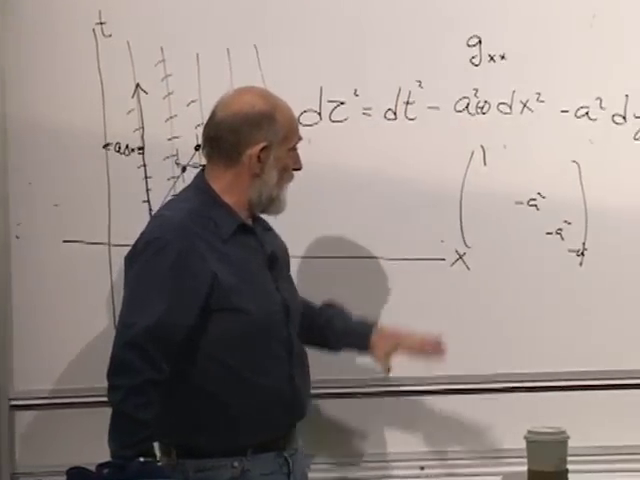
\includegraphics[width=0.82\textwidth]{lecture_01_figure_02.png}\caption{Lignes d’univers comobiles dans un Univers en expansion à une dimension spatiale, avec l’intervalle d’espace-temps correspondant.}\end{figure}

En trois dimensions spatiales, le même schéma conduit à l’extension prudente suivante\footnote{Le tableau est en partie masqué autour de 00:56:38--00:58:51. Cette forme tridimensionnelle reprend le passage oral d’une dimension spatiale à trois, ainsi que le motif diagonal visible au tableau.}\begin{equation}
d\tau^2=dt^2-a^2(t)\bigl(dx^2+dy^2+dz^2\bigr),
\end{equation}
avec une métrique diagonale
\begin{equation}
g_{\mu\nu}=\mathrm{diag}\bigl(1,-a^2,-a^2,-a^2\bigr).
\end{equation}
Les termes non diagonaux s’annulent,
\begin{equation}
g_{tx}=g_{ty}=g_{tz}=0.
\end{equation}

L’homogénéité signifie que les coefficients de la métrique peuvent dépendre du temps, mais pas de la position spatiale. L’isotropie signifie que les trois directions spatiales interviennent de la même façon.

\begin{classroomqa}\audiencequestion{Ne sommes-nous pas censés considérer \(dx\) comme une distance ?}\lecturetimestamp{01:01:18}\lecturerresponse{Non. \(dx\) n’est pas la distance. \(a\,dx\) est la distance. \(dx\) est simplement un intervalle entre repères. Pour se le représenter, on peut imaginer qu’à un moment donné, quelqu’un trace une grille de coordonnées à travers les galaxies, puis impose à cette grille de les accompagner. Par construction, la séparation en coordonnées reste fixe, tandis que la distance physique varie. On pourrait exprimer les distances dans \(x\) plutôt que dans \(a\) ; c’est une convention. Ce qui compte, c’est le produit \(a\,dx\).}\end{classroomqa}

\begin{classroomqa}\audiencequestion{Le coefficient métrique de \(dt^2\) est égal à \(1\). Est-ce également une simple convention ?}\lecturetimestamp{01:03:24}\lecturerresponse{Oui. Cela n’a en soi aucune signification physique. Si le coefficient ne dépendait que du temps, on pourrait changer de variable temporelle de sorte qu’il devienne simplement \(dt^2\). De même, on peut choisir des unités telles que \(c=1\). Ce qui n’est pas une convention ici, c’est que le coefficient ne dépend pas de la position, même s’il peut dépendre du temps.}\end{classroomqa}

\begin{classroomqa}\audiencequestion{Si l’on introduit cela dans les équations de champ d’Einstein, qu’obtient-on pour le tenseur énergie-impulsion ?}\lecturetimestamp{01:05:59}\lecturerresponse{C’est la question qui vient ensuite, mais elle relève de la dynamique et non de la discussion présente. On peut introduire cette métrique dans les équations d’Einstein et demander quelle distribution d’énergie-impulsion en ferait une solution. C’est très important, mais pour l’instant, nous parlons de géométrie, et non de dynamique.}\end{classroomqa}

\section{Ce que l’horizon nous cache}

L’Univers à grande échelle est traité comme homogène et isotrope, mais seulement de façon approximative. Il n’est certainement pas homogène à l’échelle des étoiles, des planètes, ni même des galaxies individuelles. Il n’est pas non plus exactement isotrope dans toutes les observations locales.

Un champ cultivé illustre bien la dépendance à l’échelle. À une certaine échelle, il paraît régulier ; à une échelle beaucoup plus petite, il ne l’est manifestement pas ; à une échelle supérieure à celle du champ tout entier, il cesse à nouveau de paraître homogène. Il en va de même en cosmologie. Après avoir moyenné sur de nombreuses galaxies, la distribution à grande échelle paraît à peu près uniforme. À une échelle suffisamment petite, elle ne l’est pas.

L’Univers est plus vaste que la partie que nous pouvons voir, et plus vaste encore que celle que nous pourrons jamais voir. Aux échelles que nous pouvons effectivement sonder, il est isotrope et homogène, à l’exception des variations locales. Au-delà, aucune observation directe ne nous le garantit.

\begin{classroomqa}\audiencequestion{Vous avez dit que nous ne pourrons jamais vraiment le savoir directement. Cela implique-t-il qu’il existe peut-être un moyen indirect de le découvrir ?}\lecturetimestamp{01:10:34}\lecturerresponse{Peut-être. Aujourd’hui, la plupart des chercheurs pensent que l’Univers n’est pas homogène à suffisamment grande échelle, et je parierais moi aussi dans ce sens. Mais ce pari, je ne pourrai ni le gagner ni le perdre, car, pour des raisons fondamentales, nous ne pourrons pas voir beaucoup plus loin que nous ne le faisons déjà. C’est ce qu’implique l’existence d’un horizon.}\end{classroomqa}

\begin{classroomqa}\audiencequestion{Ne pourrait-on pas utiliser la gravité pour détecter des masses au-delà de ce que l’on peut voir ?}\lecturetimestamp{01:11:53}\lecturerresponse{Non. Une masse lointaine peut simplement nous mettre en chute libre. Enfermé dans une pièce, nous sommes dans le champ gravitationnel du Soleil et nous orbitons autour de lui ; mais sans voir l’extérieur, il n’est pas facile de savoir que le Soleil est là. Seuls les effets de marée peuvent le révéler, et si la source est suffisamment éloignée, ces effets peuvent être trop faibles pour être détectés.}\end{classroomqa}

L’horizon constitue donc une limite ultime à la connaissance directe. Il affirme même, avec une quasi-certitude, que le volume de l’Univers est au moins mille fois supérieur à celui de la région que nous pourrons jamais voir, et réserve pour plus tard l’explication de cette affirmation.

\section{Fini sans bord}

Passons maintenant aux géométries fermées. La droite infinie est ouverte et non bornée. Un segment de droite est borné, au sens où il a une étendue finie. Être borné ne signifie pas avoir un bord, mais avoir une étendue finie.

Un cube avec des murs ne convient pas. Il viole l’homogénéité, car une personne près d’un mur n’est pas dans une situation équivalente à celle d’une personne éloignée des murs ; il viole aussi l’isotropie, car même une personne au centre voit des choses différentes selon la direction.

L’intérieur d’un cercle ou d’une boule ne convient pas non plus. Une personne au centre voit la même chose dans toutes les directions, mais cette symétrie ne vaut qu’en ce point particulier. Dès qu’on s’éloigne du centre, le mur est proche dans une direction et éloigné dans une autre. Pour un observateur quelconque, l’espace n’est alors ni homogène ni isotrope.

À très grande échelle, l’hypothèse de travail est que l’Univers est homogène et isotrope. C’est le principe cosmologique. Il est utile, mais n’est pas à l’abri d’une révision.

\begin{classroomqa}\audiencequestion{L’isotropie en tout point implique-t-elle l’homogénéité ?}\lecturetimestamp{01:18:57}\lecturerresponse{Oui. Si chaque observateur voit la même chose dans toutes les directions, cela implique l’homogénéité. Mais la réciproque est fausse. L’homogénéité, à elle seule, n’implique pas l’isotropie. Un Univers peut être homogène tout en ayant une direction privilégiée, par exemple s’il était rempli de flèches toutes orientées dans la même direction.}\end{classroomqa}

Le modèle borné qui convient est la surface d’une sphère sans aucun élément distinctif. Un être à deux dimensions, confiné à cette surface, trouve chaque lieu localement semblable à tous les autres, et chaque direction semblable à toutes les autres, même si le monde est fini. C’est un espace fini sans bord.

\section{Un Univers fermé unidimensionnel sur un cercle}

Pour simplifier l’algèbre, ramenons l’exemple de la sphère à une dimension spatiale : une vie sur un cercle. En une dimension, l’isotropie signifie que la gauche et la droite sont équivalentes. Le cercle possède exactement cette propriété. Choisissons un point et appelons-le \(\theta=0\). Chaque autre point est repéré par une coordonnée angulaire \(\theta\), mesurée en radians. Un point situé juste d’un côté de l’origine peut être décrit soit par un petit angle négatif, soit par un angle juste inférieur à \(2\pi\). Cette périodicité fait partie de la géométrie.

Les habitants du cercle ont accès à sa circonférence, mais pas à un rayon extérieur ni à un centre extérieur. Ils peuvent mesurer la distance totale en faisant le tour du cercle jusqu’à revenir au même point. Si l’on dessine le cercle dans un plan ambiant, on peut également introduire une quantité analogue à un rayon, mais cela relève de la représentation par plongement, et non de la géométrie intrinsèque qu’ils mesurent.

Le schéma au tableau est utile ici, car il fait figurer sur le même dessin les repères angulaires et la circonférence totale.
\begin{figure}[H]\centering
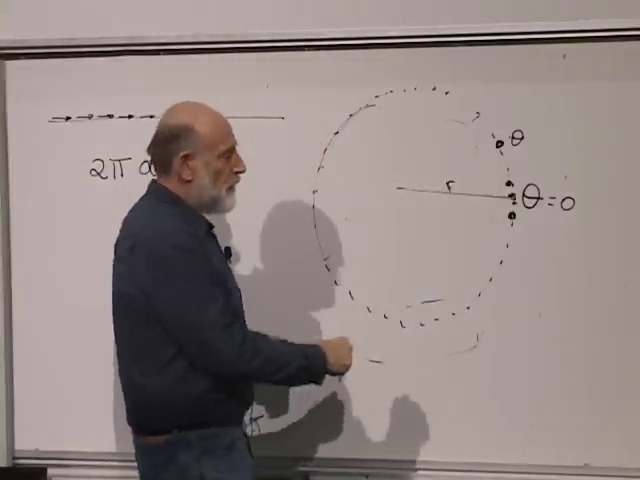
\includegraphics[width=0.82\textwidth]{lecture_01_figure_03.png}\caption{Description angulaire d’un Univers fermé à une dimension, de circonférence totale \(2\pi a\).}\end{figure}

Une convention pratique consiste à poser\footnote{Entre 01:26:40--01:29:20, la notation passe brièvement de la circonférence entière prise comme facteur d’échelle à son expression sous la forme \(2\pi a\). On utilise ici cette dernière convention, car c’est celle qui intervient ensuite dans la formule de la longueur d’arc.}\begin{equation}
L=2\pi a,
\end{equation}
où \(L\) est la circonférence totale.

Pour une petite séparation angulaire \(\Delta\theta\), la distance physique est
\begin{equation}
d=a\,\Delta\theta.
\end{equation}
En passant aux infiniment petits, on obtient
\begin{equation}
ds=a\,d\theta,
\end{equation}
et donc
\begin{equation}
ds^2=a^2\,d\theta^2.
\end{equation}
C’est la métrique locale sur le cercle.

Si \(a\) dépend du temps, l’Univers fermé à une dimension est en expansion ou en contraction. Pour une paire fixe de galaxies,
\begin{equation}
d(t)=a(t)\,\Delta\theta,
\end{equation}
d’où
\begin{equation}
\dot d=\dot a\,\Delta\theta
      =\frac{\dot a}{a}\,d.
\end{equation}
La loi de Hubble reste valable ici aussi, du moins pour les paires assez proches pour que le tour dans l’autre sens sur le cercle ne crée pas d’ambiguïté.

La métrique de l’espace-temps devient
\begin{equation}
d\tau^2=dt^2-a^2(t)\,d\theta^2.
\end{equation}
Si \(a\) est constant, la représentation de l’espace-temps est un cylindre. Si \(a\propto t\), c’est un cône. Si \(a(t)\) varie de façon plus irrégulière, la forme devient celle d’un vase.

En remontant le temps, les galaxies se rapprochent de plus en plus. S’il y avait \(360\) galaxies autour du cercle, elles seraient bien espacées à des temps tardifs, très rapprochées plus tôt, et encore davantage auparavant. Elles finiraient par ne plus être des galaxies distinctes, et, plus tôt encore, il n’y aurait même plus d’atomes distincts. Mais aucun point de l’espace n’est pour autant privilégié.

C’est la réponse la plus claire à la question de savoir où le Big Bang a eu lieu dans ce modèle. Lorsque \(a(t)\to 0\), chaque séparation \(a(t)\,\Delta\theta\) tend vers zéro. L’Univers entier se contracte partout à la fois. Les galaxies ne s’éloignent pas d’un lieu privilégié dans un espace extérieur. C’est l’échelle de la géométrie elle-même qui change. En ce sens, la réponse est : partout.

\begin{classroomqa}\audiencequestion{Vous avez dit que l’espace-temps est courbe. Le serait-il si c’était un cylindre ?}\lecturetimestamp{01:38:04}\lecturerresponse{Non. S’il s’agissait d’un cylindre, il ne serait pas courbe. C’est le cas où \(a\) est constant au cours du temps. Il ne paraît courbe que parce qu’il est représenté dans un espace de dimension supérieure. Si on le découpait, on pourrait l’aplatir sans l’étirer.}\end{classroomqa}

La discussion passe ensuite au cône. Si \(a\propto t\), la représentation de l’espace-temps est un cône. À l’écart de sa pointe, le cône est lui aussi plat au même sens intrinsèque : on peut l’ouvrir pour obtenir un plan. La pointe est différente : c’est une singularité conique.

L’étape suivante portera sur la géométrie de l’Univers sphérique, puis sur la dynamique qui détermine comment \(a(t)\) croît ou décroît.